\section{{\prg so1ion}\index{so1ion} ({\prg cfield}\index{cfield}) - a crystal field module for rare earth %%@
ions (calculate energy levels, transition matrix elements)}\label{cfield}

\subsection{Using {\prg so1ion} ({\prg Cfield}) separately}
\label{cfieldsep}

The crystal field is the electrostatic field, which is produced by the
charges of the crystal environment of a rare earth atom. It acts on the
4f electrons of the rare earth and causes magnetic anisotropy. Fig.~\ref{chrgpla} and
\ref{chrgplb} show the effect of this field on the charge distribution.
Such plots can be made by using the programs {\prg pointc\index{pointc}} to calculate
the crystal field parameters and
 {\prg chrgplt\index{chrgplt}} to plot the charge density, see section \ref{addprog}.

\begin{figure}[hb]
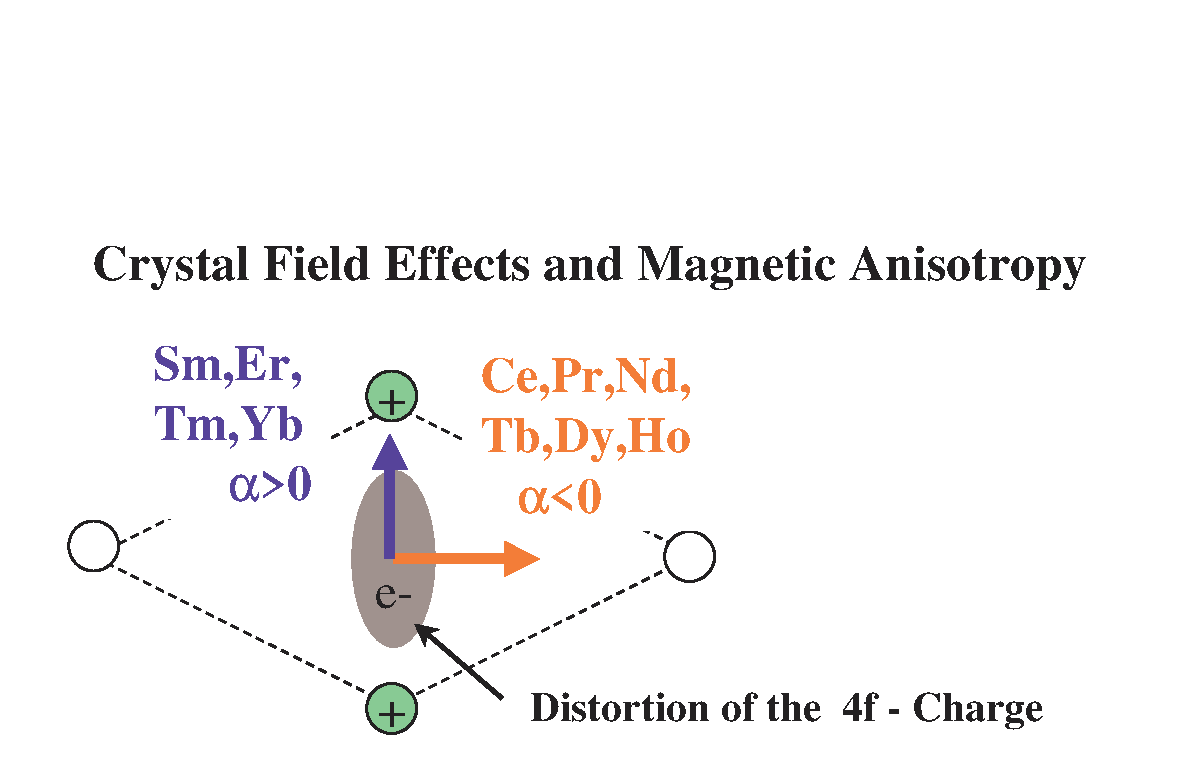
\includegraphics[angle=0,width=0.7\columnwidth]{figsrc/crystalfieldplot.eps}
\caption{\label{chrgpla}
The crystal field model: the figure shows the influence of two positive 
charges on the charge density of 4f-electrons. The
charge density is distorted by the electric field from the neighbouring atoms.
Furthermore, this distortion leads to an anisotropy of the magnetic properties
of the 4f shell. The resulting 
easy direction of the magnetic moment is shown by arrows for the different tri positive
rare earth ions.} 
\end{figure}

\begin{figure}[ht]
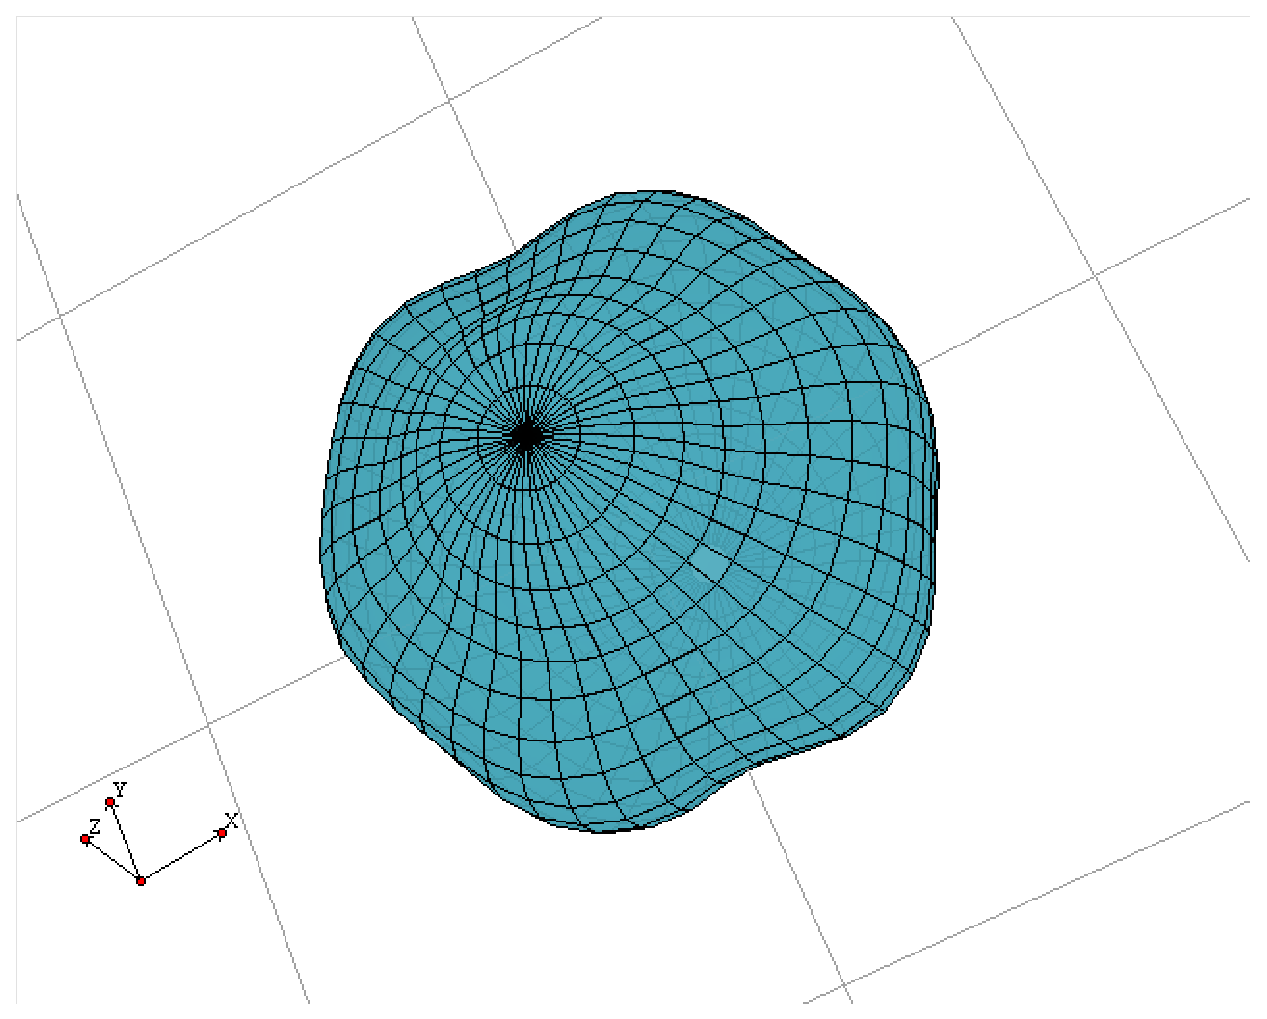
\includegraphics[angle=0,width=0.7\columnwidth]{figsrc/chrgpla.eps}
\caption{\label{chrgplb}
Calculated charge density of 4f-electrons in an orthorhombic crystal field. In
this example the charge density of a Nd$^{3+}$ ion at a temperature of 10~K was 
calculated by taking the crystal
field parameters determined by neutron spectroscopy and 
magnetic measurements in NdCu$_2$~\cite{gratz91-9297}.
[plot created by program {\prg chrgplt\index{chrgplt}+javaview}]}
\end{figure}

We will describe now, how the crystal field influence can be quantitatively evaluated
and how {\prg so1ion}\index{so1ion}  can help to do this.
Within the $|JLSm_J \rangle$ ground state multiplet of the 4f electron wave function 
the crystal field can be described by the following Hamiltonian:

\begin{equation}
\label{cfham}
 {\mathcal H}= \sum_{n,lm} B_{lm} O_{lm}({\mbf J}^n) 
	     - \sum_{n} g_{Jn} \mu_B {\mbf J}^n {\mbf H} 
\end{equation}

The first term in equ.~\ref{cfham} describes the crystal field, the second the
effect of a magnetic field (Zeeman term). The strength of the crystal field is given by the
crystal field parameters $B_l^m$. In the case of isolating materials these
parameters can be obtained by the point charge model (point charges on the 
neighbouring atoms, for details on these calculations see~\cite{hutchings64-227},
in the {\prg McPhase} suite use programs {\prg makenn} and {\prg pointc} to evaluate
the pointcharge model for a given crystal structure, see section~\ref{addprog}).
For metals the conduction electrons screen the point charges and the determination
of the crystal field is usually only possible by fits to experimental data. 
The program package {\prg McPhase} may be used to solve such crystal field problems.

A simpler way of dealing with crystal field anisotropy is to write
instead of the first term in equ.~\ref{cfham}

\begin{equation}
  \sum_s D_x^2 (J_x^s)^2 + D_y^2 (J_y^s)^2 +D_z^2 (J_z^s)^2 
\end{equation}

In order to implement a full diagonalisation of the single ion crystal field Hamiltonian
the module {\prg so1ion}\index{so1ion}({\prg cfield\index{cfield}}, written by P. Fabi n\'e Hoffmann) has %%@
been included into the program package. It  can be used separately to 
calculate crystal field problems. The program is self explaining, provided 
the user has a basic knowledge of crystal field 
theory (see e.g. the famous article by Hutchings~\cite{hutchings64-227}).
The program is started by typing {\prg so1ion}\index{so1ion} and displays help messages. 

\subsection{Example - how to evaluate the crystal field of NdCu$_2$ using {\prg %%@
so1ion}\index{so1ion}}\label{cfieldexample}

All the files described in the following procedure are available in the directory
{\prg examples/ndcu2b\_new/cf}.

A simple input file is made up in the following:

\begin{itemize}
\item The first line in the input file tells {\prg so1ion}\index{so1ion} that it should use simple input %%@
format.
\item Comment lines start with \#. 
\item The type of ion has to be given plus
several lines containing the crystal field parameters. 
\end{itemize}

It follows an example, we take the values
for NdCu$_2$ from literature~\cite{gratz91-9297}. Note that
if the crystal field parameters are not known, there are different
possibilities to obtain values, such as ab initio calculation,
point charge calculations (use module {\prg pointc\index{pointc}}) and fitting
to experimental data (see section~\ref{simannfit}).

\begin{verbatim}
#!MODULE=so1ion
#<!--mcphas.cf-->
# comment followed by
# the ion type and the crystal field parameters [meV]
 IONTYPE=Nd3+
 GJ=0.727273
# - note you can also do any pure spin problem by entering e.g. IONTYPE=S=2.5 
 B20=  0.116765                                           
 B22  =  0.134172                                           
 B40  =  0.0019225                                          
 B42  =  0.0008704                                          
 B44  =  0.0016916                                          
 B60  =  0.0000476                                          
 B62  =  0.0000116                                          
 B64  =  0.0000421                                          
 B66  =  0.0003662       
# instead of the Stevens parameters Blm 
# second order crystal field parameters Dx^2 Dy^2 and Dz^2 can be entered in meV
# - this coresponds to Hamiltonian H=+Dx2 Jx^2+Dy2 Jy^2+Dz2 Jz^2
Dx2=0.1
Dy2=0
Dz2=0.4
# the temperature in Kelvin
T= 10
# if you want you can apply a magnetic field in Tesla
Bx=0
By=0
Bz=0
\end{verbatim}

Note: you can also create an input file for so1ion with more comments for the crystal field
parameters, the type of ion etc. This is done by running {\prg so1ion}\index{so1ion} with the
option {\em -c}, i.e.: {\bf so1ion -c}, a help screen appears ...

\begin{enumerate} 
\item
The calculation of the single ion properties is 
performed using {\prg so1ion}\index{so1ion} with the option {\prg -r}, 
i.e. type the command {\bf so1ion -r filename -B} where filename
refers to the name of the single ion property file.
Files
{\prg so1ion.out} and {\prg levels.cef} (short summary, usable as input for
{\prg mcdiff\index{mcdiff}}) are generated, which contain the results of the calculation, i.e.
the diagonalisation of the Hamilton operator and the neutron scattering cross section.
The program {\prg so1ion}\index{so1ion} outputs a variety of results, such as eigenvectors and 
energies of the crystal field states. In addition it provides 
the total neutron powder cross section for each crystal field
transitions (in barn/ion) at a given temperature according to the formula

\begin{equation}
\sigma(i\rightarrow k)=4\pi \left(\frac{\hbar \gamma e^2}{mc^2}\right)^2
\frac{exp(-E_i/k_BT)}{\sum_j exp(-E_j/k_BT)} \frac{2}{3}\sum_{\alpha=x,y,z}
|\langle i|J^{\alpha}|k\rangle|^2
\end{equation}

Note: in this calculation energy and Q dependence
of the double differential scattering cross section are not considered and
integration over all energies and scattering angles has been performed.
In order to get a more realistic scattering intensity, the
form factor (giving a $Q$ dependence), the
factor $k'/k$ and the Debye Waller factor $exp(-W(Q))$ should be considered.

Here comes the output file {\prg so1ion.out}:
{\footnotesize
\begin{verbatim}
#{------------------------------------------------------------- 
#                  C F I E L D / S O 1 I O N    5.60           |
#                    A crystal field program                   |
#               __________________________________              
#              |         Peter  Hoffmann          |             
#              |    Forschungszentrum Juelich     |             
#              |Institut fuer Festkoerperforschung|             
#               __________________________________              
#    O U T P U T         Tue Aug 30 12:44:30 2011
#-------------------------------------------------------------- 
#!Temperature of the sample       T=  10.00 Kelvin                
#!Ion                    IONTYPE= Nd3+                          
#!Lande factor of the ion   gJ= 0.727273                       
#                                                              
# Total angular momentum J of the                               
#!Spin - orbit - level     J=  4.5                            
#!Electrons in 4f shell   Ne=  3                              
#-------------------------------------------------------------- 
# Parameter           :  Akq   in  meV   /a0**k                  
# (compare Hutchings Solid State Physics 16 (1964) 227, p 255 eq 5.5)                             
#!A20  =        -16.306372                                     
#!A22  =        -18.737280                                     
#                                                              
#!A40  =         -2.269445                                     
#!A42  =         -1.027477                                     
#!A44  =         -1.996875                                     
#                                                              
#!A60  =         -0.083369                                     
#!A62  =         -0.020317                                     
#!A64  =         -0.073736                                     
#!A66  =         -0.641377                                     
#-------------------------------------------------------------- 
#-------------------------------------------------------------- 
# Parameter           :  Bkq   in  meV                           
#                        Bkq are the Stevens Parameters  - see Hutchings Solid State Physics 16 (1964) 227
#!B20  =          0.116765                                     
#!B22  =          0.134172                                     
#                                                              
#!B40  =          0.001922                                     
#!B42  =          0.000870                                     
#!B44  =          0.001692                                     
#                                                              
#!B60  =          0.000048                                     
#!B62  =          0.000012                                     
#!B64  =          0.000042                                     
#!B66  =          0.000366                                     
#-------------------------------------------------------------- 
#-------------------------------------------------------------- 
# Parameter           :  Dkq   in  meV                           
#!D20 =         -36.330596                                     
#!D22 =         -17.043002                                     
#                                                              
#!D40 =         -52.832675                                     
#!D42 =          -3.782031                                     
#!D44 =          -5.556290                                     
#                                                              
#!D60 =         -20.048458                                     
#!D62 =          -0.476801                                     
#!D64 =          -1.579686                                     
#!D66 =         -10.148138                                     
#-------------------------------------------------------------- 
#-------------------------------------------------------------- 
# Parameter           :  Lkq   in  meV                           
#                        Lkq are the Wybourne Parameters - see A. Kassmann J. Chem. Phys. 53 (1970) 4118
#!L20  =        -36.330596                                     
#!L22  =        -17.043002                                     
#                                                              
#!L40  =        -52.832675                                     
#!L42  =         -3.782031                                     
#!L44  =         -5.556290                                     
#                                                              
#!L60  =        -20.048458                                     
#!L62  =         -0.476801                                     
#!L64  =         -1.579686                                     
#!L66  =        -10.148138                                     
#-------------------------------------------------------------- 
#-------------------------------------------------------------- 
# Parameter           :  Vkq   in  meV                           
# (NOT the same Vlm as in Hutchings p255 or Elliot and Stevens)
#!V20 =           0.116765                                     
#!V22 =           0.067086                                     
#                                                              
#!V40 =           0.001922                                     
#!V42 =           0.000435                                     
#!V44 =           0.000846                                     
#                                                              
#!V60 =           0.000048                                     
#!V62 =           0.000002                                     
#!V64 =           0.000021                                     
#!V66 =           0.000183                                     
#-------------------------------------------------------------- 
#-------------------------------------------------------------- 
# Parameter           :  Wkq   in  meV   /a0**k                  
#!W20 =         -16.306372                                     
#!W22 =          -9.368640                                     
#                                                              
#!W40 =          -2.269445                                     
#!W42 =          -0.513739                                     
#!W44 =          -0.998438                                     
#                                                              
#!W60 =          -0.083369                                     
#!W62 =          -0.003386                                     
#!W64 =          -0.036868                                     
#!W66 =          -0.320689                                     
#-------------------------------------------------------------- 
#-------------------------------------------------------------- 
#                Anisotropy parameters in meV.                  
#-------------------------------------------------------------- 
#         H= + Dx2 Jx ^ 2+ Dy2 Jy ^ 2+ Dz2 Jz ^ 2               
#! Dx2 =          0.10                                     
#! Dy2 =          0.00                                     
#! Dz2 =          0.40                                     
#                                                              
#-------------------------------------------------------------- 
#-------------------------------------------------------------- 
# Energy Eigenvalues are in  meV   .          	            
#--------------------------------------------------------------
#!Nr of different energy levels   noflevels= 5                 
#!Energy shift   Eshift=                       -2.6744 
#                                                              
# Because of the calibration freedom the smallest energy       
# eigenvalue is shifted to zero. You can get the energy        
# eigen-value of the applied eigen-value problem               
# by shifting the energy by the added energy value above       
#!*E( 1)=        0.0000        Degeneracy =   2 -fold            
#!*E( 2)=        2.4850        Degeneracy =   2 -fold            
#!*E( 3)=        4.5048        Degeneracy =   2 -fold            
#!*E( 4)=        7.8548        Degeneracy =   2 -fold            
#!*E( 5)=       19.1522        Degeneracy =   2 -fold            
# Them with  *  marked Energy eigenvalues have a non-          
# vanishing Matrix element of the Ground state E( 1).          
#-------------------------------------------------------------- 
#
#-------------------------------------------------------------- 
# The orthonormal characteristic Eigenvectors  |i,r>  with     
#                                                              
#             H |i,r>  = ( E  + E      ) |i,r>  , r=1 ... n    
#                           i    shift                     i   
#                                                              
#                            and                               
#                                                              
#                    <i,r|j,s> = D   D                         
#                                 ij  rs                       
#                                                              
#              D  = Kronecker- Delta function                  
#               ij                                             
#                                                              
# the |i,r> are also orthonormal .                             
# We consider in this program  Crystal Field spliting          
# at the lowest Spin-orbit-level (Ground state)                
#                                                              
# 2S+1                                                         
#     L  of the calculated Ion. The |i,r> are in               
#      J                                                       
#                                                              
# a more developed  Eigenfunction   			    
#                                                              
# system  [ | J  M   > ]               ,where                  
#                 J     M = -J,...,J                           
#                        J                                     
#                               ,                              
#              <  J  M   |  J  M  >  =  D    ,    .            
#                     J         J        M  M                  
#                                         J  J                 
#--------------------------------------------------------------
#                                                              
# I 1, 1> =     0.0414               I 4.5  -4.5>              
#          -    0.3955               I 4.5  -2.5>              
#          +    0.7083               I 4.5  -0.5>              
#          -    0.4563               I 4.5   1.5>              
#          +    0.3633               I 4.5   3.5>              
#                                                              
# I 1, 2> =     0.3633               I 4.5  -3.5>              
#          -    0.4563               I 4.5  -1.5>              
#          +    0.7083               I 4.5   0.5>              
#          -    0.3955               I 4.5   2.5>              
#          +    0.0414               I 4.5   4.5>              
#                                                              
# I 2, 1> =    -0.0402               I 4.5  -4.5>              
#          +    0.1455               I 4.5  -2.5>              
#          +    0.5713               I 4.5  -0.5>              
#          +    0.1221               I 4.5   1.5>              
#          -    0.7975               I 4.5   3.5>              
#                                                              
# I 2, 2> =     0.7975               I 4.5  -3.5>              
#          -    0.1221               I 4.5  -1.5>              
#          -    0.5713               I 4.5   0.5>              
#          -    0.1455               I 4.5   2.5>              
#          +    0.0402               I 4.5   4.5>              
#                                                              
# I 3, 1> =    -0.0255               I 4.5  -3.5>              
#          -    0.7164               I 4.5  -1.5>              
#          -    0.0601               I 4.5   0.5>              
#          +    0.6945               I 4.5   2.5>              
#          -    0.0098               I 4.5   4.5>              
#                                                              
# I 3, 2> =     0.0098               I 4.5  -4.5>              
#          -    0.6945               I 4.5  -2.5>              
#          +    0.0601               I 4.5  -0.5>              
#          +    0.7164               I 4.5   1.5>              
#          +    0.0255               I 4.5   3.5>              
#                                                              
# I 4, 1> =     0.4804               I 4.5  -3.5>              
#          +    0.5046               I 4.5  -1.5>              
#          +    0.4065               I 4.5   0.5>              
#          +    0.5712               I 4.5   2.5>              
#          -    0.1522               I 4.5   4.5>              
#                                                              
# I 4, 2> =    -0.1522               I 4.5  -4.5>              
#          +    0.5712               I 4.5  -2.5>              
#          +    0.4065               I 4.5  -0.5>              
#          +    0.5046               I 4.5   1.5>              
#          +    0.4804               I 4.5   3.5>              
#                                                              
# I 5, 1> =     0.9866               I 4.5  -4.5>              
#          +    0.1175               I 4.5  -2.5>              
#          +    0.0557               I 4.5  -0.5>              
#          +    0.0948               I 4.5   1.5>              
#          +    0.0261               I 4.5   3.5>              
#                                                              
# I 5, 2> =     0.0261               I 4.5  -3.5>              
#          +    0.0948               I 4.5  -1.5>              
#          +    0.0557               I 4.5   0.5>              
#          +    0.1175               I 4.5   2.5>              
#          +    0.9866               I 4.5   4.5>              
#                                                              
#-------------------------------------------------------------- 
#
#!magnetic moment(mb/f.u.): mx= 0.000 my= 0.000 mz= 0.000
#
#-------------------------------------------------------------- 
#                                                              
#                  M A T R I X  E L E M E N T                  
#                  S I N G L E  C R Y S T A L                    
#                                                              
#--------------------------------------------------------------
#    Only the marix elements that are non-zero are written     
#                                                              
#--------------------------------------------------------------
#                              2 |            2 |            2 
#    a  <-->  b      |<a|J |b>|  |  |<a|J |b>|  |  |<a|J |b>|  
#                         x      |       y      |       z      
#--------------------------------+--------------+--------------
#    1  <-->  1       0.002008   |  36.711411   |   0.031042   
#--------------------------------+--------------+--------------
#    2  <-->  1       1.949420   |   0.270090   |   2.638097   
#--------------------------------+--------------+--------------
#    2  <-->  2       1.517583   |   2.490016   |   8.199948   
#--------------------------------+--------------+--------------
#    3  <-->  1       1.415357   |   0.424874   |   2.727140   
#--------------------------------+--------------+--------------
#    3  <-->  2      10.148894   |   8.149608   |   0.176745   
#--------------------------------+--------------+--------------
#    3  <-->  3       9.078618   |  11.619418   |   0.380198   
#--------------------------------+--------------+--------------
#    4  <-->  1       0.009374   |   1.424032   |   1.021019   
#--------------------------------+--------------+--------------
#    4  <-->  2       2.500806   |   2.020701   |   5.118137   
#--------------------------------+--------------+--------------
#    4  <-->  3       0.239888   |   0.004479   |   4.938522   
#--------------------------------+--------------+--------------
#    4  <-->  4      26.164401   |   0.690989   |   0.070056   
#--------------------------------+--------------+--------------
#    5  <-->  1       0.710568   |   0.137243   |   0.028325   
#--------------------------------+--------------+--------------
#    5  <-->  2       2.282293   |   2.029398   |   0.008264   
#--------------------------------+--------------+--------------
#    5  <-->  3       0.057679   |   0.000101   |   0.138477   
#--------------------------------+--------------+--------------
#    5  <-->  4       3.524062   |   1.023958   |   0.749577   
#--------------------------------+--------------+--------------
#    5  <-->  5       0.060712   |   0.019195   |  38.730148   
#-------------------------------------------------------------- 
#
#
#-------------------------------------------------------------- 
#                                                              
#                  M A T R I X  E L E M E N T S                
#                    P O L Y C R Y S T A L                     
#                                                              
#--------------------------------------------------------------
#                                                              
#                             ----                2            
# Matrix element       :      >     |<i,r|J |k,s>|             
#                             ----         T                   
#                              r,s                             
#                                                              
#                                                              
# for the transition :      E  ->  E                           
#                              i      k                        
#                                                              
#--------------------------------------------------------------
#                                                              
#                         SUm rule :                           
#                                                              
#             ----                2       2                    
#             >     |<i,r|J |k,s>|  = n  --- J(J+1)            
#             ----         T           i  3                    
#             k,r,s                                            
#-------------------------------------------------------------- 
#----------------------------- 
# \ E |   |   |   |   |   |Zei|
#E \ k|E  |E  |E  |E  |E  |len|
# i \ | 1 | 2 | 3 | 4 | 5 |sum|
#----|---|---|---|---|---|---|
#| E  | 24|  3|  3|  1|   | 33|
#|  1 |.50|.24|.04|.64|.58|   |
#|----|---|---|---|---|---|---|
#| E  |  3|  8| 12|  6|  2| 33|
#|  2 |.24|.14|.32|.43|.88|   |
#|----|---|---|---|---|---|---|
#| E  |  3| 12| 14|  3|   | 33|
#|  3 |.04|.32|.05|.46|.13|   |
#|----|---|---|---|---|---|---|
#| E  |  1|  6|  3| 17|  3| 33|
#|  4 |.64|.43|.46|.95|.53|   |
#|----|---|---|---|---|---|---|
#| E  |   |  2|   |  3| 25| 33|
#|  5 |.58|.88|.13|.53|.87|   |
# ---------------------------- 
#
#
#
#-------------------------------------------------------------- 
#               Transition intensities in barn.                
#                                                              
#                                                              
#                                                              
#                                                              
# =                    - E /T     -----                        
# |                   e   i       \                   2        
# |     = const --------------     >    |<i,r|J |k,s>|         
# |             ----    - E /T    /            T               
# =             >    n e   i      -----                        
#  E -> E       ----  i            r,s                         
#   i    k       i                                             
#                                                              
#                            with                              
#                                                              
#                                                              
#                                -----                         
#                      2     2   \                    2        
#        |<i,r|J |k,s>|   = ---   >     |<i,r|J |k,s>|         
#               T            3   /             u               
#                                -----                         
#                             u = x,y,z                        
#                                                              
#                                                              
#                             und                              
#                                                              
#                                   1          2               
#                  const  = 4*pi*( --- r   g  )                
#                                   2   0   J                  
#                                                              
#                                      -12                     
#                  r      = - 0.54 * 10    cm                  
#                   0                                          
#                                                              
#--------------------------------------------------------------
#                                                              
#                       1.Sum rule :                           
#                                                 - E /T       
#                                            n   e   i         
#  ----  =            2                       i                
#  >     |         = --- * const * J(J+1) * ----------------   
#  ----  =            3                     ----     - E /T    
#   k     E -> E                            >    n  e   i      
#          i    k                           ----  i            
#                                            i                 
#--------------------------------------------------------------
#                                                              
#                       2. sum rule :                          
#                                                              
#                                                              
#            ----  =            2                              
#            >     |         = --- * const * J(J+1)            
#            ----  =            3                              
#             k,i   E -> E                                     
#                    i    k                                    
#-------------------------------------------------------------- 
#-------------------------------------------------------------- 
#!Temperature of the sample               T=   10.00 Kelvin         
#-------------------------------------------------------------- 
#!parition function            Z  =   2.12                 
#-------------------------------------------------------------- 
#!Total_magnetic_scattering_intensity =   7.94 barn            
#-------------------------------------------------------------- 
#----------------------------- 
# \ E |   |   |   |   |   |Zei|
#E \ k|E  |E  |E  |E  |E  |len|
# i \ | 1 | 2 | 3 | 4 | 5 |sum|
#----|---|---|---|---|---|---|
#| E  |  5|   |   |   |   |  7|
#|  1 |.55|.73|.69|.37|.13|.48|
#|----|---|---|---|---|---|---|
#| E  |   |   |   |   |   |   |
#|  2 |.04|.10|.16|.08|.04|.42|
#|----|---|---|---|---|---|---|
#| E  |   |   |   |   |   |   |
#|  3 |   |.01|.02|   |   |.04|
#|----|---|---|---|---|---|---|
#| E  |   |   |   |   |   |   |
#|  4 |   |   |   |   |   |   |
#|----|---|---|---|---|---|---|
#| E  |   |   |   |   |   |   |
#|  5 |   |   |   |   |   |   |
# ---------------------------- 
#
#-----------------------------------------------------------
#!Total_quasielastic_intensity =             5.68 barn           
#-----------------------------------------------------------
#                  Neutron-Energy-loss                      
#!middle_position_of_the_energy        =        2.41 meV    
#!relative_error_in_the_middl_Position  =        5.64 %      
#!Intensity_of_the_middle_position   =        0.89 barn   
#                  Neutron-Energy-Gain                 
#!middle position of the energy        =       -2.36 meV    
#!relative_error_in_the_middl_Position  =        7.74 %      
#!Intensity_of_the_middle_position   =        0.06 barn   
#-----------------------------------------------------------

#-------------------------------------------------------------- 
# Transition Energy (meV   ) vs Intensity (barn)                  
#-------------------------------------------------------------- }
  0.000  5.554803
  2.485  0.734343
  4.505  0.690467
  7.855  0.371045
 19.152  0.132449
 -2.485  0.041064
  0.000  0.103197
  2.020  0.156181
  5.370  0.081489
 16.667  0.036519
 -4.505  0.003705
 -2.020  0.014986
  0.000  0.017097
  3.350  0.004204
 14.647  0.000159
 -7.855  0.000041
 -5.370  0.000160
 -3.350  0.000086
  0.000  0.000448
 11.297  0.000088
-19.152  0.000000
-16.667  0.000000
-14.647  0.000000
-11.297  0.000000
  0.000  0.000000
\end{verbatim}
}
\item at the end of the file {\prg so1ion.out} the neutron scattering cross section of the different 
transitions is given as a list of energy vs intensity. 
In order to calculate a spectrum these results
have to be convolute\index{convolute}d with the resolution function of a neutron spectrometer. This can be 
done by the programs {\prg convolut} (available under windows only)
 or {\prg convolute\index{convolute}}. For example, the command {\bf
convolut so1ion.out 12 stp=0.05 mode=gauss fwhm=0.5} convolute\index{convolute}s the calculated neutron %%@
transitions
with a Gaussian resolution function of 0.5~meV full width half maximum. The step size of the
output spectrum is 0.05~meV. The output spectrum is contained in file {\prg so1ion.cvt}.
\item 
Use program {\prg cuthead} (available under windows only)
 to shorten the file header and {\prg display}
 to view the spectrum: {\bf cuthead 10 so1ion.cvt} and
{\bf display\index{display} 1 2  so1ion.cvt}. In order to create an image file for printing the viewed %%@
spectrum
press the save button, it creates a file {\prg display.jpg} which is shown in figure~\ref{spectrum}.
\begin{figure}[ht]
\begin{center}
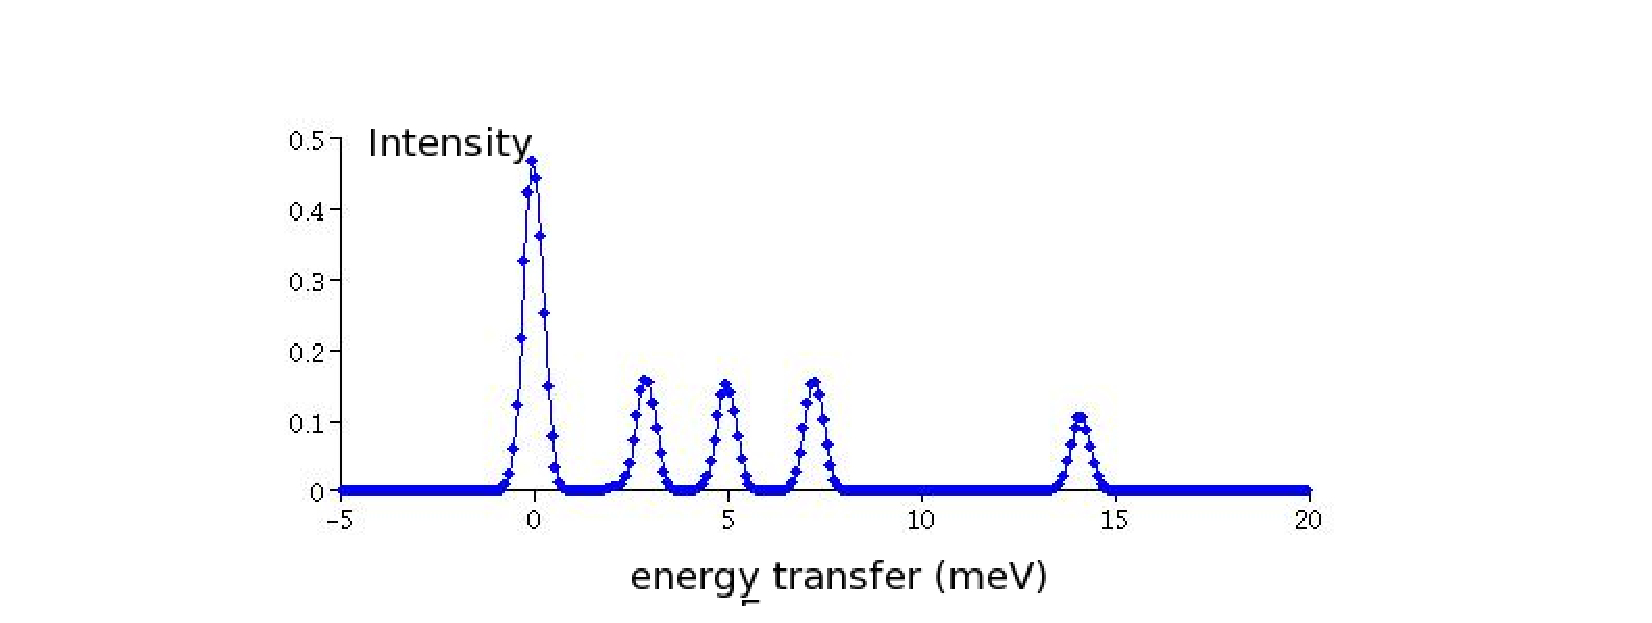
\includegraphics[angle=0,width=1.0\textwidth]{figsrc/10KCEFspectrum.eps}
\caption{\label{spectrum}
Calculated crystal field neutron spectrum of NdCu$_2$ at a temperature of 10~K.
Horizontal axis is energy transfer in meV and vertical axis is neutron intensity
in barns per meV and Nd atom.
[plot created by program {\prg display}]}
\end{center}
\end{figure}
\item In order to calculate the magnetisation for our problem (in the paramagnetic state), the
direction of the magnetic field has to be given in {\prg bkq.parmeter} and
program {\prg so1ion\index{so1ion}} has to be started with the option {\prg -m}, i.e. {\bf so1ion -m -B 0 30 %%@
10}. The
numbers denote the field range (0-30 Tesla) and the temperature (10~K). The results are written
to {\prg moment.rtplot}, fig.~\ref{moment} shows the result.
\begin{figure}[ht]
\begin{center}
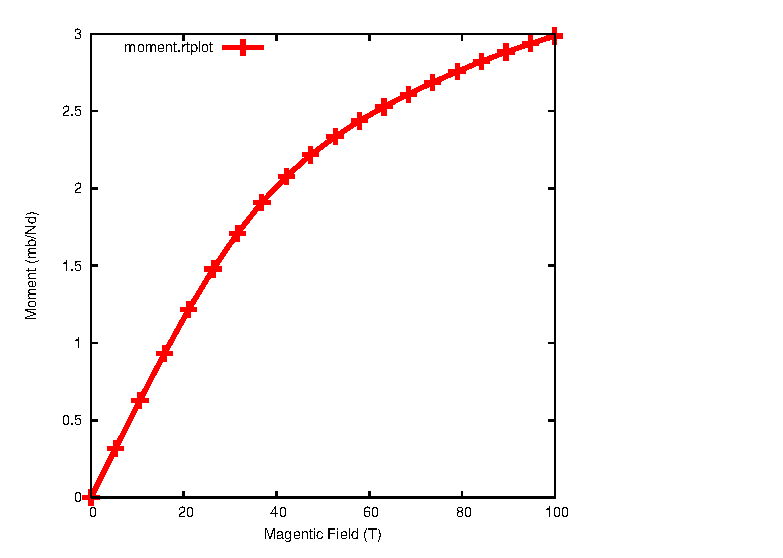
\includegraphics[angle=0,width=0.7\columnwidth]{figsrc/moment.eps}
\caption{\label{moment}
Calculated magnetic moment for field applied along $x$ direction ($c$ axis, note the
notation of the crystal field $xyz$ axes with respect to the crystal lattice is
$xyz||cab$ in our example)
 of NdCu$_2$ at a temperature of 10~K.
[plot created by program {\prg gnuplot}]}
\end{center}
\end{figure}

\item In a similar way the temperature dependence of the susceptibility can be calculated by 
{\bf so1ion -s}. 
\item The crystal field contribution to the specific heat may be calculated 
from the output file {\prg so1ion.out} using the  program {\prg cpso1ion}, e.g. {\bf cpso1ion 10 100 1 %%@
[options]}
calculates the specific heat in the temperature interval 10-100 K with a step width
of 1 K. Alternatively a comparison to experimental data can be made by {\bf cpso1ion 1 2 cpexp.dat},
where the temperatures are given in column 1 and the experimental specific heat in column
2 of file cpexp.dat. The calculated specific heat is compared to the experimental data and
a standard deviation {\em sta} is calculated and output is written to stdout.
Other quantities can be calculated using the options: -s  (calculate entropy  (J/molK) instead of cp),
-f (calculate free energy (J/mol) instead of cp),-u  (calculate magnetic energy (J/mol) instead of cp),
-z (calculate partition sum instead of cp).
Fig.~\ref{cpndcu2} shows an example.
\begin{figure}[ht]
\begin{center}
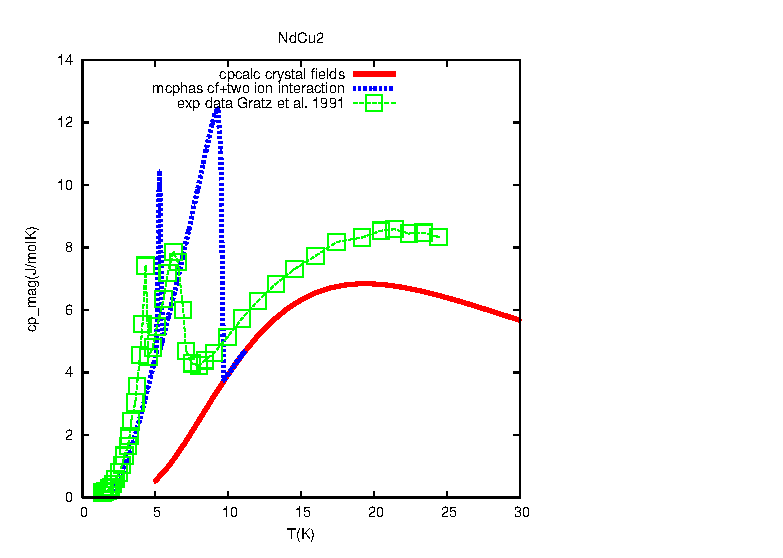
\includegraphics[angle=0,width=0.7\columnwidth]{figsrc/cpall.eps}
\caption{\label{cpndcu2}
Calculated specific heat of NdCu$_2$ in zero magnetic field as calculated
by {\prg cpso1ion} (crystal field contribution) in comparison with experimental
data~\cite{gratz91-9297}. The dashed line shows the results of a calculation,
which in addition to the crystal field takes into account the two ion interaction
and using {\prg so1ion\index{so1ion}} as a module in {\prg mcphas} - see below and chapter~\ref{runmcphas}.
[plot created by program {\prg gnuplot}]}
\end{center}
\end{figure}

\item The spin-disorder resistivity due to scattering of conduction $s$-electrons with the localised
$f$-electrons via the exchange interaction can be calculated in the first Born approximation as~\cite{raowallace},

\begin{equation} \label{eq:cfres}
\rho_{s-f}(T) = \frac{3\pi N m}{\hbar e^2 E_F} G^2(g-1)^2 \sum_{m_s,m_s',i,i'} 
      \langle m_s',i' | {\mathbf s \cdot J} | m_s, i \rangle^2 p_i f_{ii'}
\end{equation}

\noindent where $G$ is the exchange constant, $p_i$ is the Bose factor $e^{-\beta E_i}/Z$ and $f_{ii'}$ is the
Fermi function $2/(1+e^{-\beta(E_i-E_{i'})})$. The program {\prg rhoso1ion} can be used to calculate this
resistivity for magnetic ions in a crystal field. The wavefunctions $|i\rangle$ are taken from the file {\prg
levels.cef} output by {\prg so1ion}. The matrix elements of ${\mathbf s \cdot J}$ are calculated according to
the formulae of Dekker~\cite{dekker}. {\prg rhoso1ion} calculates only the sum in the above equation, however.
The constant coefficient $\rho_0=(3\pi N m/\hbar e^2 E_F) G^2(g-1)^2$ is set to unity, or may be specified using
the option {\prg --rho0} or {\prg -r}. The syntax is otherwise the same as {\prg cpso1ion}. For example, to
calculate the resistivity from 10 to 100 K in 1 K steps with $\rho_0 = 0.2$~$\Omega$.cm, the command {\bf
rhoso1ion 10 100 1 -r 0.2} can be used. Alternatively, for comparison with data, {\bf rhoso1ion 1 2 rhoexp.dat
-r 0.2} can be used. Note that as the temperature dependence of the resistivity in this case is mainly a
function of the Bose and Fermi functions, at high temperatures where all $2J+1$ crystal field levels are
thermally occupied, the resistivity will saturate to a value $\rho_0 J(J+1)$.

\end{enumerate}

\vspace{1cm}
{\em Exercises:}
\begin{itemize}
\item Use {\prg so1ion\index{so1ion}} to calculate the energies, eigenvectors and
transition matrix elements (for inelastic
neutron scattering) for Nd$^{3+}$ in an orthorhombic crystal field.
Use the parameters given in section~\ref{cf1ion}.
\end{itemize}



\subsection{Using {\prg so1ion\index{so1ion}} as a module in {\prg McPhase} and {\prg McDisp}}
\label{cf1ion}


The use 
 of {\prg so1ion\index{so1ion}} as a module in {\prg mcphas} is necessary in order to 
 go beyond the capabilities of {\prg so1ion\index{so1ion}} (for instance the calculation
 of magnetisation or specific heat or if the exchange interaction
 given in equations~(\ref{hamilton}) and (\ref{multipolehamilton})
  shall be taken into account).  

\subsubsection{Module Tasks:}


As a single ion module, {\prg so1ion\index{so1ion}} provides to {\prg mcphas} the magnetic properties
of a single rare earth ion subject to the crystal field. Its main duty is
to calculate the magnetic moment given an effective magnetic field. 
To be more explicit - given the effective magnetic field $H^s_{eff}$ by {\prg mcphas}
 the module {\prg so1ion\index{so1ion}}
 diagonalises the crystal field and Zeeman Hamiltonian (\ref{cfze}) of the
 ion $n$:

\begin{equation}\label{cfze}
 {\mathcal H_n}=  B_l^m O_{lm}({\mbf J}^n) 
	     -  g_{Jn} \mu_B {\mbf J}^n {\mbf H^n_{eff}} 
\end{equation}

and calculates the expectation value of the angular momentum
 $\langle \mbf J^n \rangle$
according to

\begin{equation}
\langle \mbf J^n \rangle =
\sum_{\Gamma} p_{\Gamma} \langle \Gamma | \mbf J^n | \Gamma \rangle
\end{equation}

with 

\begin{eqnarray}
p_{\Gamma}&=&\frac{\exp(-E_{\Gamma}/kT)}{z}\\
z&=&\sum_{\Gamma} \exp(-E_{\Gamma}/kT)
\end{eqnarray}

Here $z$ is the partition sum, $|\Gamma\rangle$ the eigenstate corresponding to
the eigenvalue $E_{\Gamma}$ of the Hamiltonian (\ref{cfze}). 
\footnote{In addition to $\langle \mbf J_i \rangle$ the module also returns
the partition sum $z$ and the magnetic energy $u=\sum_{\Gamma} p_{\Gamma} E_{\Gamma}$.}

\subsubsection{Module Usage:}
 

The program {\prg mcphas} (-calculation of the magnetic phase diagram) 
requires a single ion
property input file of the same format as given above in
section~\ref{cfieldexample} (also for each ion in the
crystallographic unit cell):

\begin{itemize}
\item The first line in the single ion property file tells {\prg mcphas} that the module
{\prg so1ion\index{so1ion}} should be used for this ion. 
\item Comment lines start with \#. 
\item The type of ion has to be given plus
several lines containing the crystal field parameters. 
\end{itemize}

It follows a simple  example (for more complicated examples see section \ref{sifile} and 
{\prg mcphas.cf1} in the 
directory {\prg examples/ndcu2b\_new}):


\begin{verbatim}
#!MODULE=so1ion
#<!--mcphas.cf-->
# comment followed by
# the ion type and the crystal field parameters [meV]
 IONTYPE=Nd3+
# - note you can also do any pure spin problem by entering e.g. IONTYPE=S=2.5 
 B20=  0.116765                                           
 B22  =  0.134172                                           
 B40  =  0.0019225                                          
 B42  =  0.0008704                                          
 B44  =  0.0016916                                          
 B60  =  0.0000476                                          
 B62  =  0.0000116                                          
 B64  =  0.0000421                                          
 B66  =  0.0003662                                          
\end{verbatim}


\begin{description}
\item [Note:] 
In order to use {\prg so1ion\index{so1ion}} as a module in {\prg McPhase} a convention for
the orientation of the $xyz$ coordinate system (of the crystal field) relative
to the crystal axis $abc$ has to be made:
 The axes convention adopted in module {\prg so1ion} for the crystal field parameters
is - $\mbf a||x$, $\mbf b||y$ and $\mbf c||z$. Note that if you use the
module {\prg cfield}, the choice is more unconventional:$\mbf a||y$, $\mbf b||z$ and $\mbf c||x$
Tools for rotating crystal field parameters are described in appendix~\ref{rotateBlm}.

The reason for
this unique choice is to make it possible to treat quadrupolar interactions - the 
generalisation of bilinear interactions to these higher order interactions
is much easier in this a first glance very unconventional axes convention.
Furthermore, for the higher order interactions it is also convenient to
adopt the same orientation of the coordinate system for each atom.


{\small
{\bf Information for experienced users:} the first line in the single ion property file
can either refer to  one of the standard
single ion property modules (e.g. Kramers ground state
doublet \#!MODULE=kramers, full crystal field \#!MODULE=so1ion) or a shared library file, which will be %%@
loaded
dynamically into the program at runtime 
 - for a description
of this file see section~\ref{sifile}.
}
